\chapter{STUDI DAN EKSPLORASI APACHE SPARK}
\label{chap:studi dan eksplorasi}

Pada bab ini, akan dijelaskan eksplorasi yang dilakukan pada Spark. Studi dan eksplorasi dilakukan untuk mengetahui lebih tentang fungsi-fungsi RDD pada Spark, cara instalasi, Spark \textit{shell}, dan Spark UI.

\section{Instalasi Apache Spark}

Berikut adalah tahap-tahap untuk melakukan instalasi Apache Spark. Apache Spark yang  digunakan adalah Apache Spark versi 2.3.1. Spark dapat berjalan di atas berbagai sistem operasi seperti Windows dan UNIX systems (Contoh Linux, macOS). Sebelum memulai instalasi Apache Spark, terdapat beberapa kebutuhan yang harus dipenuhi seperti instalasi Java dan Scala. Berikut adalah langkah-langkah untuk memastikan bahwa kebutuhan minimal telat terpenuhi:

\begin{itemize}

\item Pastikan bahwa Java telah di-\textit{install} dan versi java yang di-\textit{install} adalah setidaknya 8+ karena Spark berjalan pada versi minimal Java 8+. Berikut adalah command untuk memastikan java telah di-\textit{install}:

\begin{verbatim}
$ java -version
Java(TM) SE Runtime Environment (build 1.8.0_112-b15)                                                                   Java HotSpot(TM) 64-Bit Server VM (build 25.112-b15, mixed mode) 
\end{verbatim}


\item Pastikan bahwa Scala telah di-\textit{install} dengan versi minimal 2.11.x. Berikut adalah perintah untuk memastikan bahwa Scala telah di-\textit{install} dengan versi yang benar:

\begin{verbatim}
$ scala -version
Scala code runner version 2.11.6 -- Copyright 2002-2013, LAMP/EPFL
\end{verbatim}

\end{itemize} 

Bila Java dan Scala belum di-\textit{install} pada komputer, berikut adalah langkah-langkah instalasi Java dan Scala untuk kebutuhan Spark:

\begin{itemize}

\item Berikut adalah perintah-perintah untuk menginstal Java menggunakan terminal pada sistem operasi Linux:

\begin{verbatim}
$ sudo apt-get update
$ sudo apt-get install openjdk-8-jdk
\end{verbatim}

\item Berikut adalah perintah-perintah untuk menginstal Scala menggunakan terminal pada sistem operasi Linux:

\begin{verbatim}
$ sudo apt-get update
$ sudo apt-get install scala
\end{verbatim}

\end{itemize}


Instalasi dapat dilakukan ketika syarat-syarat di atas telah dipenuhi. Berikut adalah langkah-langkah instalasi Apache Spark:

\begin{enumerate}

\item Unduh versi Spark yang diinginkan  dari https://spark.apache.org/downloads.html

\item \textit{Extract} Spark tar dengan \textit{command} berikut:

\begin{verbatim}
$ cd /home/user/Downloads/ 
$ tar xvf spark-2.3.1-bin-hadoop2.7.tgz 
$ mv spark-2.3.1-bin-hadoop2.7 /home/user/spark-2.3.1-bin-hadoop2.7 
\end{verbatim}

\item Lakukan konfigurasi \textit{environment variable} untuk Spark. Ubah file .bashrc dengan menambahkan perintah berikut pada file:

\begin{verbatim}
export SPARK_HOME=/home/user/spark-2.3.1-bin-hadoop2.7
export PATH=$PATH:/home/user/spark-2.3.1-bin-hadoop2.7/bin
\end{verbatim}

\item Jalankan perintah berikut untuk memastikan perubahan telah terjadi pada file .bashrc:

\begin{verbatim}
source .bashrc
\end{verbatim}

\item Ketika Spark di-\textit{install} dengan benar, maka kita dapat menjalankan spark-shell seperti pada (Gambar~\ref{fig:sparkshell}). Berikut adalah perintah untuk menjalankan spark-shell:

\begin{verbatim}
$ $SPARK_HOME/bin/spark-shell
\end{verbatim}

\begin{figure}[H]
    \centering  
    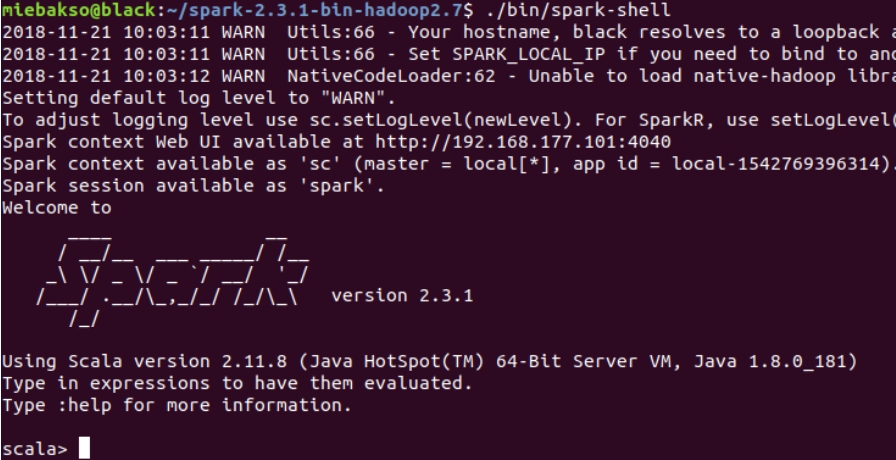
\includegraphics[scale=0.7]{sparkshell}  
    \caption[{\it Spark Shell} ]{{\it Spark Shell}} 
    \label{fig:sparkshell} 
\end{figure}

\end{enumerate}


\section{Eksplorasi Spark Shell}

Bagian ini  menjelaskan percobaan untuk menghitung jumlah setiap kata pada file \textit{text} README.md. Spark \textit{shell} digunakan untuk menjalankan perintah-perintah agar Spark bisa menghitung jumlah setiap kata yang ada pada file \textit{text} tersebut. Setiap kata yang sama akan dijumlahkan. Pada bagian ini akan digunakan \textit{transformation} dan juga \textit{action}.

\begin{figure}[H]
    \centering  
    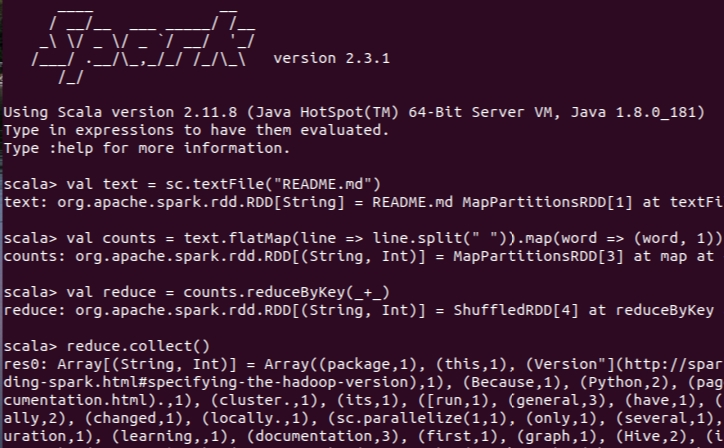
\includegraphics[scale=0.7]{wordcount}  
    \caption[{\it Word Count} ]{{\it Word Count}} 
    \label{fig:wordcount} 
\end{figure}

Berdasarkan Gambar~\ref{fig:wordcount}, berikut adalah langkah-langkah percobaan yang dilakukan:

\begin{enumerate}

\item Jalankan spark shell dengan \textit{command} berikut pada terminal:

\begin{verbatim}
$ ./bin/spark-shell
\end{verbatim}

\item Buat \textit{text} RDD dari sumber eksternal, yaitu file README.md. \textit{Command} di bawah digunakan untuk membuat RDD dari file eksternal:

\begin{verbatim}
scala> val text = sc.textFile("README.md") 
\end{verbatim}

Dapat dilihat bahwa RDD bertipe \textit{String} telah sukses dibuat.

\begin{verbatim}
text: org.apache.spark.rdd.RDD[String] = README.md MapPartititonsRDD[1]...
\end{verbatim}


\item Gunakan operasi \textit{transformation} flatMap() untuk memecah kalimat menjadi kata-kata. Setelah itu, setiap kata akan dijadikan pasangan \textit{key} (kata) dan \textit{value} (kata,1). Berikut adalah perintah yang harus dijalankan:

\begin{verbatim}
val counts = text.textflatMap(line => line.split(" ")).map(word => (word, 1))
counts: org.apache.spark.rdd.RDD[(String, int)] = ShuffledRDD[3] ...
\end{verbatim}

\item Hitung jumlah setiap kata dengan menggunakan operasi reduceByKey(). Operasi reduceByKey() akan menjumlahkan kata dengan \textit{key} yang sama. Contoh perintah dapat dilihat dibawah:  

\begin{verbatim}
val reduce = counts.reduceByKey(_+_)
reduce: org.apache.spark.rdd.RDD[(String, int)] = ShuffledRDD[4] ...
\end{verbatim}

\item Ambil hasil operasi sebelumnya dengan menggunakan operasi collect() yang merupakan sebuah \textit{action}. Berikut adalah perintah yang harus dijalankan:

\begin{verbatim}
reduce.collect()
//Hasil
res0: Array[(String, Int)] = Array((package,1), (Python,2), .....
\end{verbatim}

\end{enumerate}

\section{Instalasi Apache Spark pada \textit{Multi-Node Cluster}}

Seperti yang telah disebutkan sebelumnya, Apache Spark dapat diterapkan \textit{ multi-node cluster}. Berikut adalah langkah-langkah yang harus dilakukan:

\begin{enumerate}

\item Tambahkan entri dalam file host \textit{master} dan \textit{slave}. \textit{Master} merupakan komputer utama dan \textit{slave} merupakan komputer pekerja. Berikut adalah perintah yang harus dijalankan: 

\begin{verbatim}
$ sudo gedit /etc/hosts
\end{verbatim}

Tambahkan IP \textit{master} dan juga \textit{slave} pada file.

\begin{verbatim}
<MASTER-IP> master
<SLAVE1-IP> slave1
<SLAVE2-IP> slave2
<SLAVE3-IP> slave3
\end{verbatim}

\item Install Java pada setiap \textit{master} dan \textit{slave}, jangan lupa untuk memastikan versi Java yang di install. Berikut adalah perintah untuk menginstal Java:

\begin{verbatim}
$ sudo apt-get update
$ sudo apt-get install default-jdk
\end{verbatim}

Pastikan versi Java yang di-\textit{install} dengan perintah berikut:

\begin{verbatim}
$ java -version
\end{verbatim}

\item instal Scala pada setiap master dan slave, jangan lupa untuk memastikan versi Scala yang di-\textit{install}.

\begin{verbatim}
$ sudo apt-get update
$ sudo apt-get install scala
\end{verbatim}

Pastikan versi Scala yang di-\textit{install} dengan perintah berikut:

\begin{verbatim}
$ scala -version
\end{verbatim}

\item Setelah melakukan instalasi Scala dan Java, \textit{install} Open SSH Server-Client pada \textit{master}. Berikut adalah perintah yang harus dijalankan:

\begin{verbatim}
$ sudo apt-get install openssh-server openssh-client
$ ssh-keygen -t rsa -P 
\end{verbatim}

\item Lakukan konfigurasi SSH pada \textit{slave} dan juga \textit{master}. Salin \texttt{.ssh/id\_rsa.pub} milik \textit{master} kepada \texttt{.ssh/authorized\_keys} untuk \textit{master} dan juga \textit{slave}.

\item Setelah itu, kita akan mengunduh dan menginstal Spark pada setiap \textit{slave} dan \textit{master}. Berikut adalah langkah-langkah yang diikuti:
\begin{verbatim}
Unduh versi Spark yang diinginkan pada https://spark.apache.org/downloads.html
\end{verbatim}
Ekstrak Spark dengan perintah berikut:
\begin{verbatim}
$ tar xvf spark-2.3.0-bin-hadoop2.7.tgz
$ sudo mv spark-2.3.0-bin-hadoop2.7 /home/user/spark
\end{verbatim}

\item Setelah selesai menginstal Spark, kita harus mengubah file .bashrc.
Buka file bashrc dengan command berikut:
\begin{verbatim}
$ sudo gedit .bashrc 
\end{verbatim}
Tambahkan baris berikut pada file .bashrc:
\begin{verbatim}
export PATH = $PATH:/home/user/spark/bin
\end{verbatim}
Jalankan perintah berikut untuk memastikan perubahan telah terjadi pada file .bashrc:
\begin{verbatim}
source .bashrc
\end{verbatim}

\item Lakukan konfigurasi pada \textit{master} dengan mengubah file spark-env.sh. Berikut adalah perintah-perintah yang harus dijalankan
\begin{verbatim}
$ cd /home/user/spark/conf
$ cp spark-env.sh.template spark-env.sh
$ sudo gedit spark-env.sh
source .bashrc
\end{verbatim}
Tambahkan baris berikut pada file tersebut:
\begin{verbatim}
export SPARK_MASTER_HOST='<MASTER-IP>'
export JAVA_HOME=<Path_of_JAVA_installation>
\end{verbatim}
Kemudian edit file slaves pada /home/user/spark/conf dengan perintah berikut:
\begin{verbatim}
$ sudo gedit slaves
\end{verbatim}
Tambahkan baris berikut pada file tersebut:
\begin{verbatim}
master
slave1
slave2
slave3
\end{verbatim}

\item Jalankan spark \textit{cluster} dengan perintah berikut:

\begin{verbatim}
$ cd /usr/local/spark
$ ./sbin/start-all.sh
\end{verbatim}
Untuk memberhentikannya masukan perintah berikut:
\begin{verbatim}
$ ./sbin/start-all.sh
\end{verbatim}


\end{enumerate}

\section{Percobaan Spark Submit}

Pada percobaan ini, kita akan mencoba mengumpulkan sebuah jar kepada spark-submit. Aplikasi yang dibuat harus memiliki konfigurasi Spark dan diubah menjadi jar untuk dikumpulkan kepada spark-submit. Aplikasi yang dibuat akan membaca file yang disediakan dan menghitung jumlah kata yang ada. Sebelum melakukan percobaan, terdapat beberapa kebutuhan yang harus dipenuhi. Berikut adalah kebutuhan-kebutuhan yang harus dipenuhi:

\begin{enumerate}

\item \textit{Install} dan sudah melakukan konfigurasi untuk Scala, Java, dan Spark.

\item \textit{Install} IntelliJ IDEA dari https://www.jetbrains.com/idea/. IntelliJ IDEA adalah \textit{integrated development environment} untuk pengembangan perangkat lunak. Intellij dirancang oleh JetBrains untuk meningkatkan produktivitas developer. Intellij memiliki beberapa fitur seperti integrasi dengan GitHub, \textit{smart code completion}, \textit{intelligent refactorings}, dan lain-lain.

\item SBT merupakan \textit{ open-source build tool} untuk Scala dan Java. SBT sangat mirip dengan Maven dan Ant. SBT memiliki beberapa fitur seperti \textit{Dependency management}, \textit{incremental testing},  \textit{incremental compilation},  dan lain-lain.

Berikut adalah langkah-langkah instalasi SBT:

\begin{verbatim}
$ echo "deb https://dl.bintray.com/sbt/debian /" | sudo tee -a /etc/apt/sources.list.d/sbt.list
$ sudo apt-key adv --keyserver hkp://keyserver.ubuntu.com:80 --recv 2EE0EA64E40A89B84B2DF73499E82A75642AC823
$ sudo apt-get update
$ sudo apt-get install sbt
\end{verbatim}


\end{enumerate}

Setelah kebutuhan telah terpenuhi maka percobaan dapat dimulai. Berikut adalah langkah-langkah percobaan:

\begin{enumerate}

\item Pertama, buka IntelliJ dan buat sebuah project SBT seperti pada Gambar ~\ref{fig:intelij}.

\begin{figure}[H]
    \centering  
    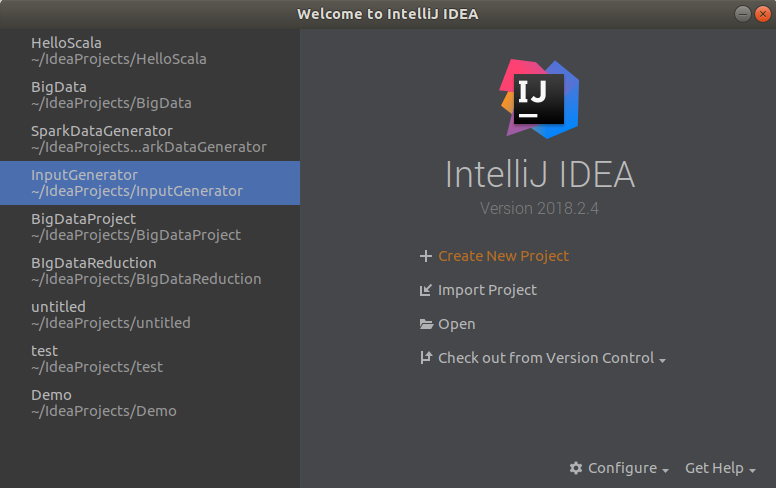
\includegraphics[scale=0.35]{intelij}  
    \caption[ItelliJ IDEA]{ItelliJ IDEA} 
    \label{fig:intelij} 
\end{figure}

Setelah itu, pilih proyek Scala yang menggunakan sbt. Tekan tombol \textit{next} seperti pada Gambar~\ref{fig:newproject}.

\begin{figure}[H]
    \centering  
    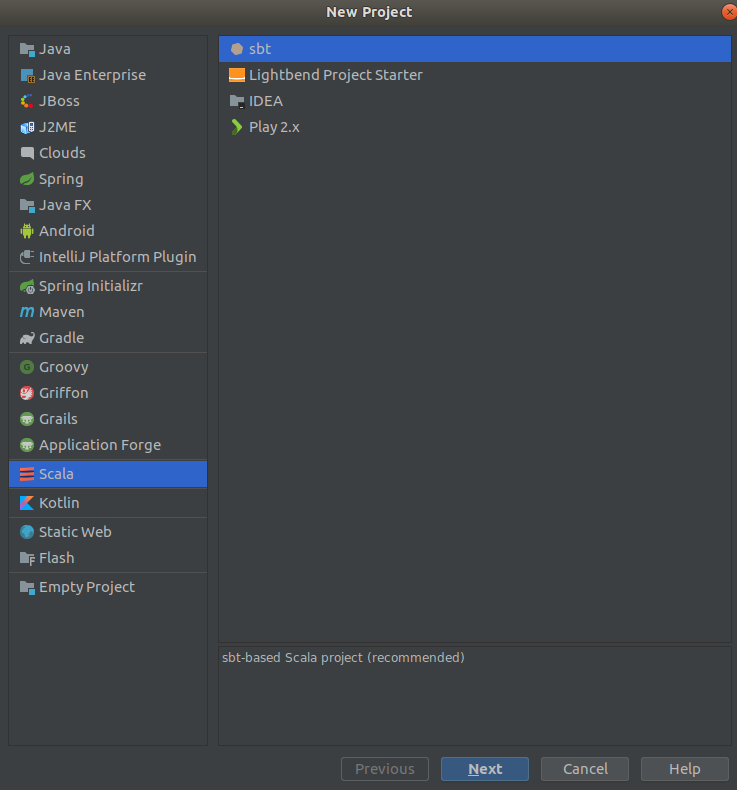
\includegraphics[scale=0.4]{newproject}  
    \caption[Proyek sbt]{Proyek sbt} 
    \label{fig:newproject} 
\end{figure}

Kemudian, beri nama proyek dengan nama WordCount dan pilih versi Sbt, Java, dan Scala yang sesuai seperti pada Gambar~\ref{fig:projectconfig}. 

\begin{figure}[H]
    \centering  
    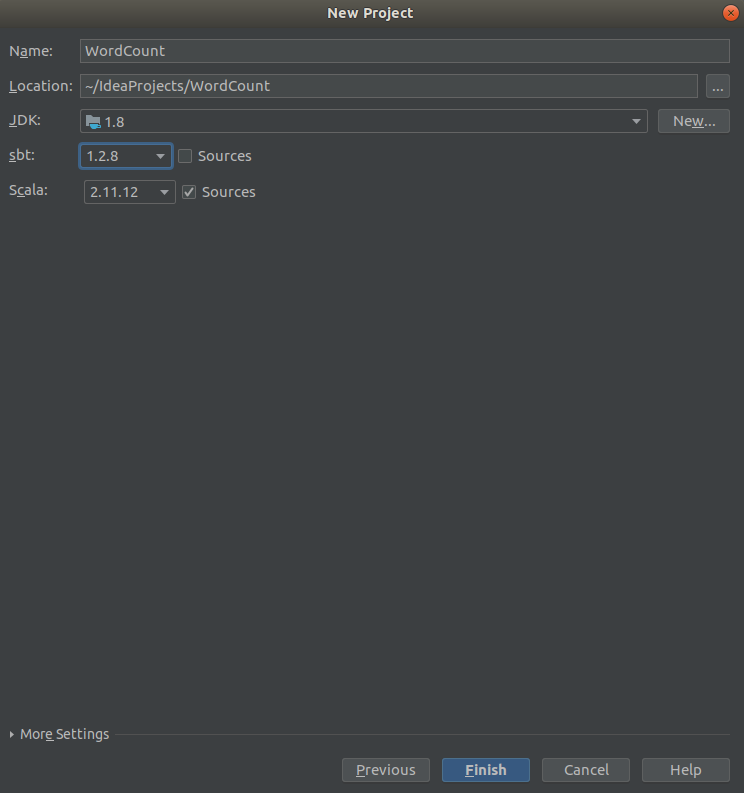
\includegraphics[scale=0.4]{projectconfig}  
    \caption[Konfigurasi proyek]{Konfigurasi proyek} 
    \label{fig:projectconfig} 
\end{figure}

Hasil dari pembuatan proyek baru pada IntelliJ akan terlihat seperti pada Gambar\ref{fig:structure}.

\begin{figure}[H]
    \centering  
    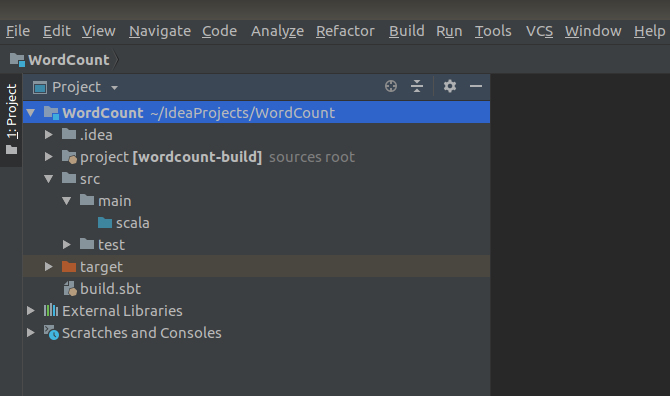
\includegraphics[scale=0.5]{structure}  
    \caption[Struktur proyek ]{Struktur proyek} 
    \label{fig:structure} 
\end{figure}

\item Setelah membuat proyek baru, buka file build.sbt dan tambahkan baris seperti pada Gambar\ref{fig:sbt}.


\begin{figure}[H]
    \centering  
    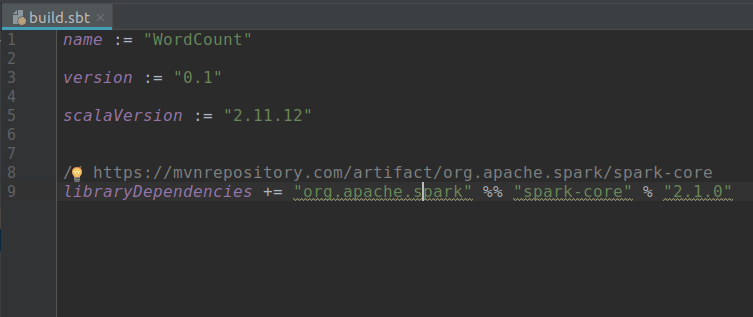
\includegraphics[scale=0.5]{sbt}  
    \caption[Konfigurasi sbt]{Konfigurasi sbt} 
    \label{fig:sbt} 
\end{figure}

\item Tambahkan \textit{object} WordCount pada proyek seperti pada Gambar\ref{fig:object}.

\begin{figure}[H]
    \centering  
    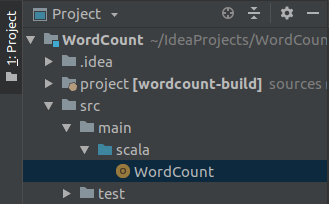
\includegraphics[scale=0.7]{object}  
    \caption[\textit{object} WordCount]{\textit{object} WordCount}.
    \label{fig:object} 
\end{figure}


Setelah itu, tambahkan kode berikut seperti contoh \ref{code:wordcount}.

\begin{lstlisting}[language=Scala, caption=WordCount.scala, label={code:wordcount}]
package main.scala
import org.apache.spark.{SparkConf, SparkContext}
object WordCount {
    def main(args: Array[String]):Unit = {
        val conf = new SparkConf()
        conf.setMaster("local")
        conf.setAppName("Test")
        val sc = new SparkContext(conf)
        val textFile = sc.textFile("/path/to/input.txt")
        val counts = textFile.flatMap(line => line.split(" "))
            .map(word => (word,1))
            .reduceByKey(_+_)
        counts.saveAsTextFile("/path/to/output.txt")
    }
}
\end{lstlisting}

\item Jalankan perintah 'sbt package' untuk meng-\textit{compile} kode menjadi \textit{executable} JAR seperti pada Gambar\ref{fig:jar}. Hasil keluaran dapat dilihat pada Gambar\ref{fig:sbtpackage}.

\begin{figure}[H]
    \centering  
    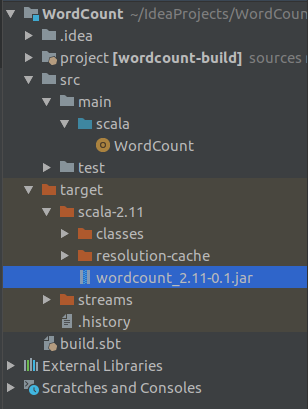
\includegraphics[scale=0.5]{jar}  
    \caption[JAR]{JAR} 
    \label{fig:jar} 
\end{figure}

\begin{figure}[H]
    \centering  
    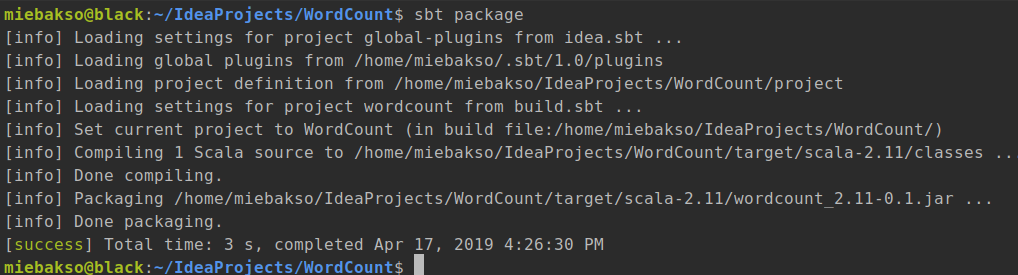
\includegraphics[scale=0.5]{sbtpackage}  
    \caption[Hasil perintah 'sbt package']{Hasil perintah 'sbt package'} 
    \label{fig:sbtpackage} 
\end{figure}

\item Setelah berhasil membuat JAR, masukan file JAR kepada \textit{spark-submit} seperti pada Gambar \ref{fig:sparksubmit}. Berikut adalah perintah yang harus dijalankan: 

\begin{verbatim}
$ cd $SPARK_HOME
$ ./bin/spark-submit --class main.scala.WordCount --master local[1] \
/home/miebakso/IdeaProjects/WordCount/target/scala-2.11/wordcount_2.11-0.1.jar 
\end{verbatim}

\begin{figure}[H]
    \centering  
    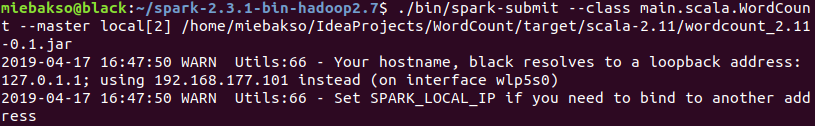
\includegraphics[scale=0.6]{sparksubmit}  
    \caption[Penggumpulan JAR kepada \textit{spark-submit}]{Penggumpulan JAR kepada \textit{spark-submit}} 
    \label{fig:sparksubmit} 
\end{figure}

Hasil tahap-tahap proses dari program dapat dilihat pada Spark UI dengan membuka alamat yang digaris bawah biru pada Gambar \ref{fig:linkui}

\begin{figure}[H]
    \centering  
    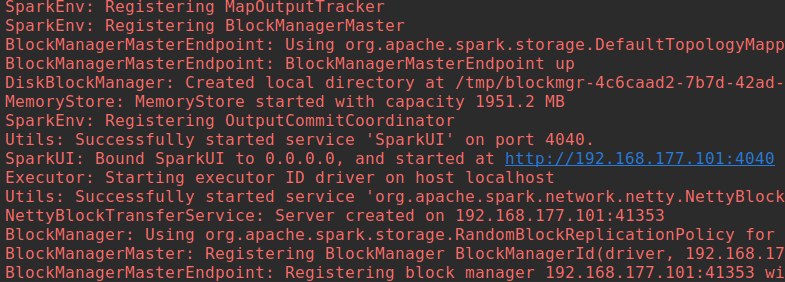
\includegraphics[scale=0.6]{linkui}  
    \caption[Alamat Spark UI]{Alamat Spark UI} 
    \label{fig:linkui} 
\end{figure}

Spark UI menggambarkan tahap-tahap proses program. Tampilan dari Spark UI dapat dilihat pada Gambar \ref{fig:sparkui}.
\begin{figure}[H]
    \centering  
    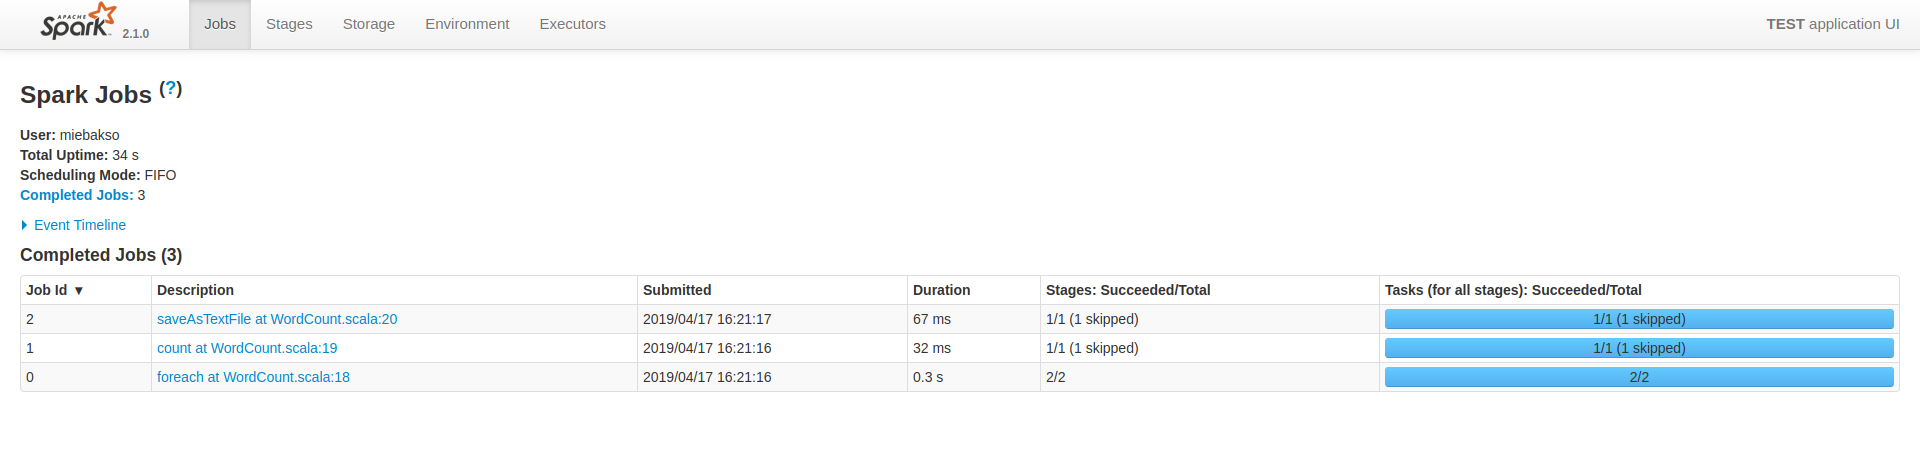
\includegraphics[scale=0.25]{sparkui}  
    \caption[Spark UI]{Spark UI} 
    \label{fig:sparkui} 
\end{figure}





 
\end{enumerate}
